\documentclass{article} % For LaTeX2e
\usepackage{nips11submit_e,times}
%\documentstyle[nips10submit_09,times,art10]{article} % For LaTeX 2.09
\usepackage{graphicx} 


\RequirePackage{amsfonts}
\RequirePackage{amsmath}
\newtheorem{definition}{Definition}
\newtheorem{theorem}{Theorem}
\newtheorem{proof}{Proof}
\newtheorem{conjecture}{Conjecture}

\newcommand{\suchthat}{ \mathrel{\ooalign{$\ni$\cr\kern-1pt$-$\kern-6.5pt$-$}}}

\title{A Hybrid Approach for Optimal Hierarchical Reinforcement Learning}


\author{
Hai-Feng Kao
Department of Computer Science\\
University of British Columbia\\
\texttt{haifeng@cs.ubc.ca}
}

% The \author macro works with any number of authors. There are two commands
% used to separate the names and addresses of multiple authors: \And and \AND.
%
% Using \And between authors leaves it to \LaTeX{} to determine where to break
% the lines. Using \AND forces a linebreak at that point. So, if \LaTeX{}
% puts 3 of 4 authors names on the first line, and the last on the second
% line, try using \AND instead of \And before the third author name.

\newcommand{\fix}{\marginpar{FIX}}
\newcommand{\new}{\marginpar{NEW}}

%\nipsfinalcopy % Uncomment for camera-ready version

\begin{document}


\maketitle

\begin{abstract}
Model-based reinforcement learning methods make an efficient use of samples by 
building the model of the environment and simulating from it.
Compared to model-free methods, it usually takes fewer samples to converge to the optimal policy.
Despite of the efficiency, model-based methods
suffer from the curse of dimensionality due to the fact that
the size of planning envelope grows exponentially with the number 
of features. In this paper, we propose an approximated model-based
approach to tackle this problem. By combining with 
hierarchically optimal recursive Q-learning (HORDQ) under 
the hierarchical reinforcement learning framework, we show that
the proposed approach converges to the optimal policy even when
the model is arbitrarily wrong.
\end{abstract}


%contribution: if the approximated model is good, it will converge faster than flat SARSA. 
%if not, it still converge eventually
%model-based approach is hard, they cannot figure out the correct Q value because the design of the model is biased
%model-free is ok because Gt doesn't require a model
%A fail safe mechanism to ensure that approximated model-based approach may
%converge to optimal policy even when the model is approximated
%converge even when our model is biased
%if the model worked--> converge to optimal policy fast
%if not, it will converge to the optimal policy anyway
%1. Motivate the purpose: 
   %0. the factered model is intrinsticly biased for non factored one
   %1. the power of model based approach (introduce the previous work and the lack of approximation)
   %2. previous work on approximated model based approach (2 actions and n steps is O(2^n))
   %2. previous work on model-based HRL
   %3. previous work on hybrid approach (no guaranntee on a approximated model) (all coarse to fine approach)
   %4. introduce HORDQ
   %5. the problem of HORDQ: worse than flat Q without transfer, our sol: add internal reward
   %6. our contribution: show that the important property is that it will converge to optimal policy for any planner
   %7. our contribution: combine with model-based approach (HORDQ is userful when we combine it with some approximated model)
   %8. a natural extension: use high internal reward in the beginning and decrease it in the end
   %Hierarchical Policy Gradient Algorithms
%2. Introduction on MAXQ
%3. Biased model
%4. HORDQ
%4.1. Pseudo reward
%5. the leaf cover
%6. add all primitive actions and the necessary (and the price)
%5. show the optimality
%5.1. the offline case (not depend on Andre's proof)
%5.2. the online case (the conjecture status, how about chaning policy (value iteration)? --> define a new mdp)
%5.3. TD equation
%6. The three optimality (recursive optimality is not possible(model is approximated) bottom node recursive optimal is bad (always select get passenger),hierarchical optimality is impossible. the only hope is optimal)
%7. the respect of the hierarchy
%8. The experiment (school bus problem)
%9. The optimality cannot be achieved with recursive optimal (random planner with MAXQ --> the problem of existing approximation approach)
%10. With HORDQ, it is possible but slow (random planner with HORDQ)
%11. with appropriate penality it can be faster
%12. it works well if sometimes the model works and sometimes don't --> the agent can learn when to trust the planner (main contribution)
%12. why we don't use TAXI domain
%13. say that only model-free node has the Qe term
%14. do I need to include algorithm
%15. DO NOT use planning envelope
%16. We can construct Hierarchy automatically from HexQ or manually design it (make my approach applicable to any problems)
%17. We can use GLIE policy to prove its convergence
%18. Pseudo reward

%show that hierarchical optimal policy becomes optimal policy when all primitive actions
%are available for all s in s_i
%the conjecture problem->another motivation why we need to focus on primitive actions
%The intuition is that the update rule for [] is actually the standard flat SARSA algorithm except that different subtasks have their own table.
%The intuition on QE (make subagent to rebel the hierarchy)
%Show that after modification, the hierarchical optimality can be achieved and it is equal to optimality

\section{Introduction}

%hard to learn a model: non-smothness of probability and reward function, factoered assumtion, size of planning envelope
%cannot give any optimality guarantees,

The methods of model-based reinforcement learning learns a effective policy by 
by learning the model from samples and simulating experiences
from the model. It generally requires less samples to find the optimal policy. 
However, when the state space is too large, we cannot build the exact model anymore.
Instead, we have to approximate the model with function approximation techniques. Few works address 
the problem of model-based reinforcement learning with approximation in an online setting.

Factored Markov decision process (FMDP) has been applied successfully to solve large 
problems \cite{ApproxFactor} \cite{SPUDD}. However, these methods require the prior knowledge
on transition and reward functions of the problem, which may be not be available in practice.
Degris and Sigaud \cite{ApproxTree} extended Dyna \cite{Dyna} with the approximation of decision trees.
Sutton et al. \cite{ApproxDyna} introduced linear Dyna -- a combination 
of Dyna and linear function approximation. 
Instead of enumerating all states, which is impossible for large problems, they
use Dyna style planning. Given the current state and policy, 
their methods predict the feature of next state and reward by function approximation
techniques. Despite the difficulty of correct prediction, their methods are biased 
for stochastic environment. It is possible to have
several possible next states given the same state and policy in a stochastic environment.
If we predict the most likely one, we cannot find the optimal policy because of the bias in our model.

On the other hand, model-free methods learn Q-function directly. It does not 
learn the model and it does not have simulating steps.  
The existing linear function approximation algorithms for model-free methods \cite{LSTD99} are effective. 
They are the method of choice if we want to apply reinforcement learning 
to large problems.

In this work, we combine model-based and model-free methods with the hierarchical 
reinforcement learning (HRL) framework. We propose a simple approximated model which 
may improve the learning efficiency. However, the model is too simple to represent
complex problems and it may fail to learn the optimal policy. We show that by combining with 
hierarchically optimal recursive Q-learning (HORDQ) \cite{HORDQ}, which is a model-free method, we can 
guarantee that the overall policy will converge to the optimal one even when our model
fails to approximate the problem and becomes arbitrarily wrong. 

Our approach assumes the task hierarchy for a MDP is given. The hierarchy can either be 
designed manually or learned by automatic hierarchy discovery techniques\cite{HexQ}

%Our contribution includes: 
%1. Derived a condition that the hierarchical optimal policy is equal to the optimal policy
%2. Under the same condition, some subtasks policies do not affect the optimality of overall policy
%3. A fail safe mechanism to ensure that approximated model-based approach may

%TODO: state that it is fine if we do not learn the transition function or reward function correctly

We are not the first who try to combine different RL methods within the HRL framework.  
Ghavamzadeh and Mahadevan \cite{HybridPolicy} combined value function-based RL and policy gradient RL to handle
continuous MDP problems. In Cora's thesis \cite{Vlad}, he   
incorporate model-based, model-free and the Bayesian active learning to the MAXQ framework.
Nevertheless, these methods seek recursive optimality in the learning process, 
thus they fail to satisfy any optimality condition when one of the subtasks
is failed to find its optimal policy.
On the contrary, our method learns the optimal policy without the requirement that 
all of the policy of subtasks need to be optimal. It is more robust and allows us to incorporate approximated
approaches into the same framework.


%say the benefit of model-based RL (peter's model based HRL, 
%illustrate the problem of model-based RL

%show that it can be resolved by HRL
%say other HRL work, but no one addresses the optimality with biased model

%At higher level, we use model-based approach to do the planning on a coarser state representation. 
%At lower level, model-free approach is used....
%[Ditterich did that as well]
%Instead of focusing on safe state abstraction, we are more interested in the unsafe one.
%The state of real world problem can be very large and complicated, we may 
%not always find a safe abstracition. In this work, we show that the 
%optimality can still be achieved if 1. 2. 
%[CMU TR][] some uses (unsafe) corasers state at higher level, but none of them 
%provide any guarrante the optimality when the coarser representation are
%not safe, 

%None of the previous approaches 

\section{Model formulation}

\begin{definition} Markov decision process is formalized as a tuple $<S, A, P, R>$, where
\begin{itemize}{}
\item $S$ is a finite set of states of the environment.
\item $A$ is a finite of actions.
\item The transition function $P:S \times A \times S \rightarrow [0, 1]$ defines a probability distribution over the possible next states. 
\item The reward function $R:S \times A \rightarrow \mathbb{R}$ defines the reward after executing a certain action at a certain state.
\end{itemize}
\end{definition}

Given a state of the environment, a policy $\pi: S \times A$ tells what action should be performed at that state. 
The value function $V^{\pi}: S \times \mathbb{R}$ is the expected cumulative reward when executing
policy $\pi$ from state $s$.

The value function satisfies the Bellman equation:
\begin{equation}
    V^{\pi}(s) = \sum_{s'}P(s'|s, \pi(s))[R(s, \pi(s)) + \gamma V^{\pi}(s')],
    \label{eq:V}
\end{equation}
where $\gamma \in [0, 1]$ is the discount factor which discounts the future reward to the present value.

Similarly, we define the action-value function (or Q function) as:
\begin{equation}
    Q^{\pi}(s, a) = \sum_{s'}P(s'|s, a)[R(s'|s, a) + \gamma Q^{\pi}(s', \pi(s'))].
    \label{eq:Q}
\end{equation}
The Q function is the expected cumulative reward after executing action $a$ at state $s$ and following
$\pi$ thereafter.

%\begin{equation}
    %Q^{\pi}(s, a) = \sum_{s', N}P(s', N|s, a)[R(s', N|s, a) + \gamma^N Q^{\pi}(s', \pi(s'))].
    %\label{eq:SMDPQ}
%\end{equation}
%Now lets us extends action set $A$ to include composite actions.

%The transition function $P$ and $R$ are modified to include the time to accomplish each composite action:
%\begin{equation}
    %R(s, a) = \sum^{\infty}_{k=0} \gamma^k r_k
%\end{equation}

%The value function needs to be modified as:
%\begin{equation}
    %V^{\pi}(s) = \sum_{s'}P(s'|s, \pi(s))[R(s, \pi(s), t) + \gamma^N V^{\pi}(s')],
%\end{equation}
%where $N$ is the number of steps for the action $\pi(s)$ to finish its execution.
%A question arises since we do not know the actual time to finish executing each composite action.
%Let's set $gamma=1$ from now on.
%TODO: (how MaxQ solve it?).

In this work, we follow the MaxQ hierarchy defined in \cite{MaxQJ}:
\begin{definition}
    Given a MDP $M$, the hierarchical reinforcement learning decomposes $M$ into a finite
    set of subtasks $M = {M_0, M_1, \dots, M_n}$, where $M_0$ is the root subtask. 
    Each subtask is defined by 3 tuples $<T_i, A_i, \tilde{R}_i>$. 
    \begin{itemize}{}
    \item $T_i$ is a termination predicate. It partitions state space $S$ into active states $S_i$ and
                terminal states $T_i$. If subtask $M_i$ enters any terminal states, it terminates immediately
                and return the control to the parent subtask. A parent subtask cannot execute the subtask
                $M_i$ if the current state belongs to $T_i$.
    \item $A_i$ is a set actions which are available to subtask $M_i$. An action can be either primitive or composite.
                If it is composite, it pass execution to the corresponding subtask. No recursive calls 
                are allowed in the hierarchy.
    \item $\tilde{R}_i$ is the pseudo reward function 
    \end{itemize}
\end{definition}
A hierarchical policy $\pi = \{\pi_1, \pi_2, \dots, \pi_n\}$ is a set which contains all subtask policies. 
The subtask policy $\pi: S_i \rightarrow A_i$ maps an active state to one of the actions to execute.

%Andre and Russell \cite{OptimalQ} extends MaxQ framework to be hierarchical optimal.
%They defined $Q_E(i, s, \pi(s))$ as:
%\begin{equation}
    %Q_E^{\pi}(i, s, \pi(s)) = \Sigma_N \Sigma_{x \in T_i}P(x, N| s, \pi(s)) \gamma^N Q^{\pi}(x, \pi(x)).
    %\label{eq:QE}
%\end{equation}
%$Q_E^{\pi}(i, s, \pi(s))$ is the expected cumulative reward after $i$-th node follows 
%policy $\pi$ at state $s$ and terminates at some point.

%In theorem ?, we show that if we modify the hierarchy and let some subtasks to have access all primitive actions, 
%the hierarchical optimal policy is equal to the optimal policy.

\section{Optimality with Biased Model}
\begin{figure}[t]
\begin{center}
    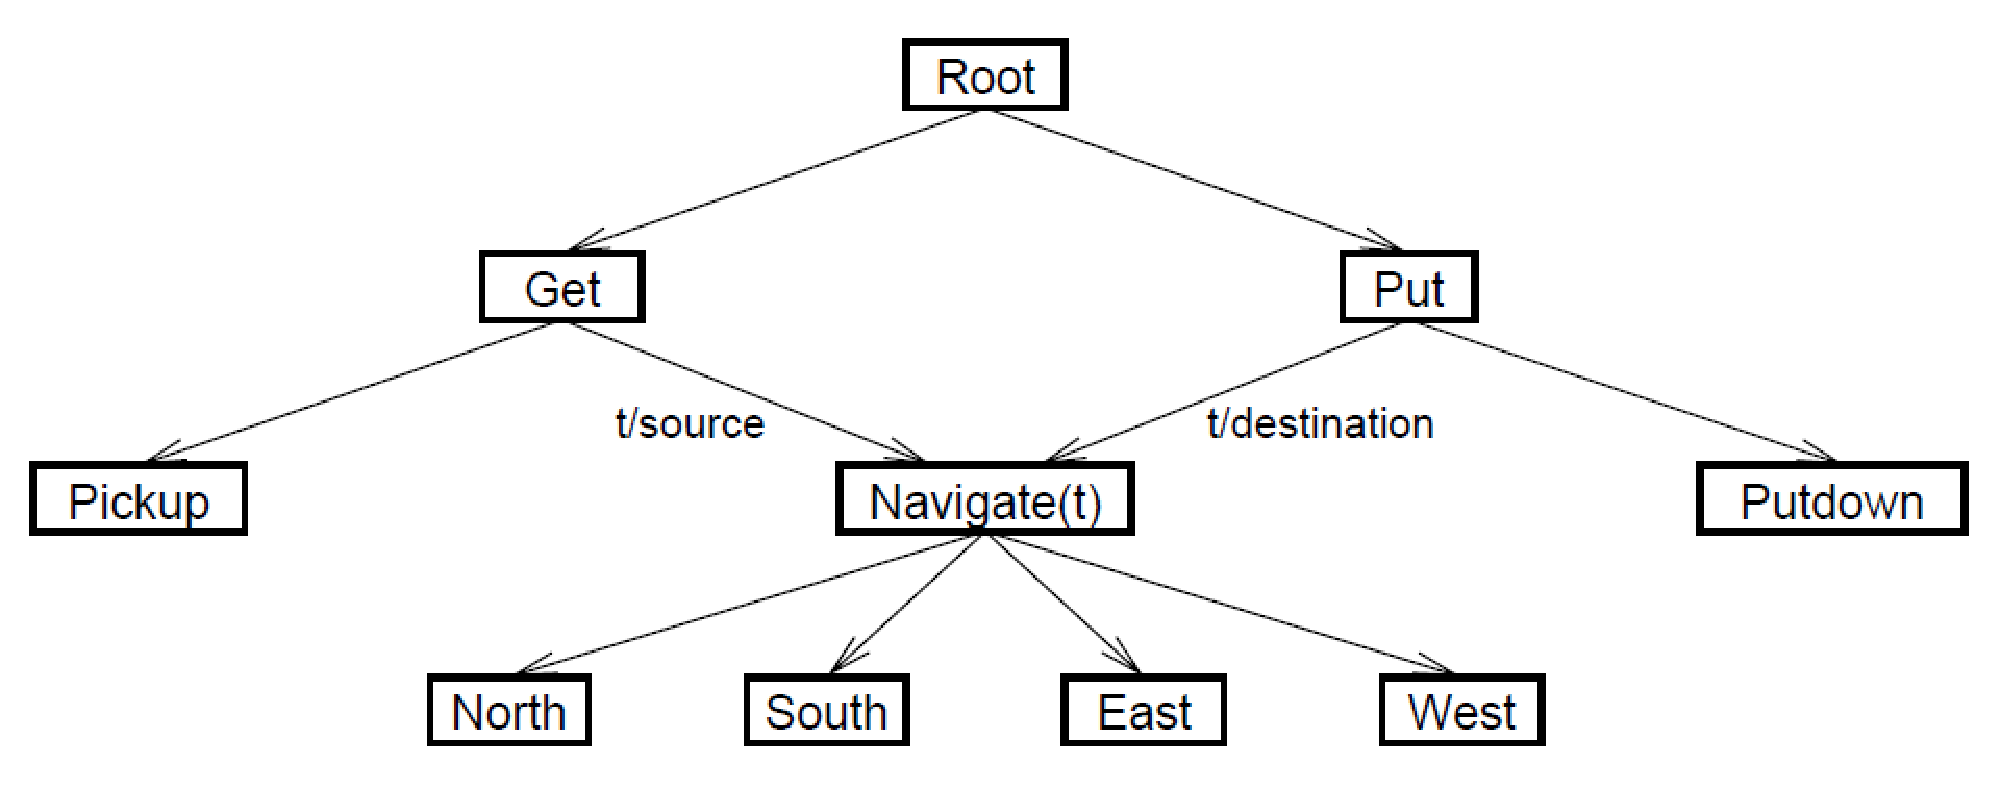
\includegraphics[width=4in] {TaxiHierarchy.eps}
\end{center}
\caption{The task hierarchy of taxi domain \cite{MaxQJ}.}
\label{fig:taxi}
\end{figure}

%The primary contribution of this work is to show that by combining model-based and 
%model-free approaches, we can still achieve optimality even when the model is biased.

We illustrate our idea with the task hierarchy (Fig. \ref{fig:taxi}) of taxi problem introduced by Dietterich\cite{MaxQJ}.
Assume Root subtask is suboptimal and always choose Get subtask even when 
the passenger is in the taxi, we can guarantee the optimality if Get subtask
learns to deliver the passenger to his destination when the passenger is in the taxi.
Likewise, if Put subtask learns to pickup the passenger when he is not in the taxi, 
we will have the optimal policy because not matter what decision is made 
by Root subtask, the passenger can always be picked up and delivered to the destination.

However, it cannot be done without the modification of the hierarchy. In the original hierarchy, 
Get subtask has no access to Putdown action. Even though Get subtask arrive the destination,
it will never complete the task. We need to modify the hierarchy to let Get subtask be
able to solve the problem on its own. A way to achieve it is to let Get subtask have access
to all primitive actions. By doing this, the exploration space of Get subtask increases
because of additional actions. It will increase 
the time to learn the optimal policy. However, if the model-based method can effectively increase
the convergence rate, the time to learn the optimal policy might still decrease.

%We can only guarantee optimality by adopting HORDQ for certain positions
%in the hierarchy. The "positions" are defined by the following definition:

\begin{definition}
    $C(H) = \{M_1, M_2, \dots, M_k\}$ is a leaf cover of hierarchy $H$ 
    if there are no subtask $M_i \notin C(H)$ which has access to a primitive action.
    Furthermore, $TC(H)$ is a total leaf cover if all primitive actions are available for every 
    subtasks $M_i \in TC(H)$.
\end{definition}

A leaf cover contains the subtasks which are required to learn the optimal policy.
We can always find a leaf cover of hierarchy by including all subtasks which have access
to primitive actions. We can convert a leaf cover to a total leaf cover by 
adding all primitive actions to the subtasks. 
Consider the task hierarchy in taxi domain in Figure \ref{fig:taxi},
if we add Pickup and Putdown actions to Navigate subtask and remove the access of these actions from Get and Put subtasks,
we get a total leaf cover by including Navigate subtask in it. Another way is to let Navigate, Get and Put subtasks
have access to all six primitive actions and include these subtasks in the total leaf cover. 

Our objective is to prove that we can learn the optimal policy if we use HORDQ \cite{HORDQ} on the subtasks which 
belong to a total leaf cover.

HORDQ decomposes Q-value as:
\begin{align}
    \label{eq:HordQ}
    Q^{\pi}(i, s, a) = E[\sum_{t=0}^{\infty}\gamma^t r_t &= E[\sum_{t=0}^{N_1 - 1}\gamma^t r_t] + E[\sum_{t=N_1}^{N_2 - 1}\gamma^t r_t] + E[\sum_{t=N_2}^{\infty}\gamma^t r_t]\\
                    &= Q_r^{\pi}(i, s, a) + Q_c^{\pi}(i, s, a) + Q_e^{\pi}(i, s, a),
\end{align}
where $N_1$ is the number of primitive actions to finish action $a$, $N_2$ is the number of primitive actions 
to finish subtask $M_i$. 

%TODO: $Q_r$ 


%The node queries its children node to get the value of $V^{\pi}(a, s)$.
$Q_r^{\pi}$ can be computed by:
\begin{equation}
    Q_r^{\pi}(i, s, j) = 
    \left\{\begin{array}{ll}
        Q_r^{\pi}(j, s, \pi_j(s)) + Q_c^{\pi}(j, s, \pi_j(s))& \mbox{if j is composite} \\
        \Sigma_{s'} P(s'|s, j)R(s'|s, j) & \mbox{if j is primitive} \\  
    \end{array} \right.
    \label{eq:Qr}
\end{equation}
%In our example, to compute $Q^{\pi}(MaxRoot, s, GotoExit)$, "MaxRoot" node would query 
%"MaxExit" node to get $V^{\pi}(GotoExit, s)$.

The $Q_c^{\pi}(i, s, a)$ can be computed:
\begin{equation}
    Q_c^{\pi}(i, s, a) = \sum_{s', N} P_{s_i}^{\pi}(s', N|s, a)\gamma^N[Q_r^{\pi}(i, s', \pi_i(s')) + Q_c^{\pi}(i, s', \pi(s'))].
    \label{eq:Qc}
\end{equation}


%Note that $P(s'|s, \pi(s))$ and $V^{\pi}(a, s)$ are provided by the child Max nodes.
And $Q_e^{\pi}$:
\begin{equation}
    Q_e^{\pi}(i, s, a) = \sum_{s', N} P_{x_i}(s', N|s, a)\gamma^N[Q^{\pi}(k, s', \pi_k(s'))],
    \label{eq:Qe}
\end{equation}
where $k$ is the index of subtask which executes subtask $M_i$.

However, to use $Q(k, s', \pi_k(s')$ in equation \ref{eq:Qe} to update $Q_e^{\pi}$ may not be correct, because the model
of the parent subtask $M_k$ might be a biased one. Only the Q value of subtask $M_i \in C(H)$ is trustworthy.
Hence, we have to modify equation \ref{eq:Qe} as:

\begin{equation}
    Q_e^{\pi}(i, s, a) = \sum_{s', N} P_{x_i}(s', N|s, a)\gamma^N[Q^{\pi}(o_c^{\pi}(i, s'), s', a')],
    \label{eq:OptQe}
\end{equation}
where $a' = \pi_j(s')$, and $j = o_c^{\pi}(i, s')$ is the next subtask in $TC(H)$ which will be executed. 
Note that the property of leaf cover ensures that we can always find such $j$ before any primitive
action is executed. %TODO: (why?).



\begin{theorem}
    If $TC(H)$ is a total leaf cover of hierarchy $H$, and $Q^{\pi}$, $Q_r^{\pi}$, $Q_c^{\pi}$ and $Q_e^{\pi}$ satisfy equation
    %TODO:
    10, 
    \ref{eq:Qr}, \ref{eq:Qc}, and \ref{eq:OptQe} separately, $Q^{\pi}$ satisfies Bellman equation:
    $Q^{\pi}(i, s, a) = \sum_{i', s', N}P(i', s', N|s, a)[R(s'|s, a) + \gamma^N Q^{\pi}(i', s', \pi_{i'}(s'))]$
\end{theorem}

%TODO: not all s are defined in Q(i, s, a) (focus on si instead of all i)
%TODO: what if pi_c_bar may change for every step?
%TODO: what if pi_c_bar is not deterministic
%TODO: write down the Q learning algorithm and the model-based one
%TODO: why Q^*(i, s, a) = Q^*(s, a) shows that hierarchical pi is the optimal policy
%TODO: any rigorous property for leaf cover?
%TODO: do I use all assumption for the theorem?
%TODO: the relationship between HORDQ and my approach
%TODO: provide the reason why we need to acceess all primitive action (because of the dumb and never learn planner)
%TODO: show that I can convert any MDP problem to hierarchy one, thus we can always combine approximated model-based approach with HORDQ.

\begin{theorem}
    If $TC(H)$ is a total leaf cover, we have $Q^*(i, s, a) = Q^*(s, a), \forall i \in \mathbb{C}(H)$
\end{theorem}
\textbf{Proof:} Let $\pi_{\bar{\mathbb{C}}}: \mathbb{C}(H) \times S \rightarrow \mathbb{C}(H)$ be the policy to invoke
the next subtask $j = \pi_{\bar{\mathbb{C}}}(i, s)$ which belongs to $\mathbb{C}(H)$. It is determined
by the policy of subtasks which do not belong to $\mathbb{C}(H)$ and terminate predicate $T_i$. Follow Bellman's equation, we have:
\begin{align}
    Q^{\pi}(i, s, a) &= \sum_{s'} P^{\pi}(\pi_{\bar{\mathbb{C}}}(i, s'), s'|i, s, a) [R(s', s, a) + \gamma Q^{\pi}(\pi_{\bar{\mathbb{C}}}(i, s'), s', \pi_i(s'))]\\
    &=\sum_{s'}P^{\pi}(\pi_{\bar{\mathbb{C}}}(i, s')| i, s, a, s') P(s' | i, s, a)  [R(s', s, a) + \gamma Q^{\pi}(\pi_{\bar{\mathbb{C}}}(i, s'), s', \pi_i(s'))]\\
    &\mbox{since $\pi_{\bar{\mathbb{C}}}$ is a deterministic policy}\\
    &=\sum_{s'} P(s' | s, a) [R(s', s, a) + \gamma Q^{\pi}(\pi_{\bar{\mathbb{C}}}(i, s'), s', \pi_i(s'))]
    \label{eq:MaxIrr}
\end{align}

Compare to the Bellman equation of the flat MDP:
\begin{equation}
    Q^{\pi_f}(s, a) = \sum_{s'}P(s'|s, a)[R(s', s, a) + \gamma Q^{\pi_f}(s', \pi_f(s'))].
    \label{eq:bellman}
\end{equation}

The equations \ref{eq:MaxIrr} and \ref{eq:bellman} are identical except for the Q values.
Due to uniqueness of Bellman equation, if $\pi_i(s) = \pi_f(s), \forall s$, we will have $Q^{\pi_f}(s, a) = Q^{\pi_f}(i, s, a)$. 
If $\pi_i(s) = \pi^*_f(s)$, $Q^*(s, a)$ is a solution and also an optimal solution (why?) of equation \ref{eq:MaxIrr}.
Thus we have $Q^*(i, s, a) = Q^*(s, a)$. \textbf{Q.E.D.}

The previous equations assume we have complete knowledge about of problem and can compute
the Q function with dynamic programming. If we do not have the knowledge, we can
use temporal difference learning instead:
%TODO: the discount term compared the Bellman 
\begin{equation}
    \tilde{Q}_r(i, s, j) \leftarrow
    \left\{\begin{array}{ll}
    (1 - \alpha)\tilde{Q}_r(i, s, j) + \alpha R(s'| s, j)  & \mbox{if j is primitive} \\
    \tilde{Q}_r(j, s, \pi_j(s)) + \tilde{Q}_c(j, s, \pi_j(s)) & \mbox{if j is composite} \\
    \end{array} \right.
    \label{eq:TdQr}
\end{equation}
\begin{equation}
    \tilde{Q}_c(i, s, j) \leftarrow
    \left\{\begin{array}{ll}
    (1 - \alpha)\tilde{Q}_c(i, s, j) + \alpha \gamma^N[\tilde{Q}_r(j, s', \pi_j(s')) + \tilde{Q}_c(i, s', \pi_i(s'))]  & \mbox{if $s' \in S_i$} \\
    (1 - \alpha)\tilde{Q}_c(i, s, j) + \alpha \gamma^N[\tilde{Q}_r(j, s', \pi_j(s'))]  & \mbox{if $s' \in T_i$} \\
    \end{array} \right.
    \label{eq:TdQc}
\end{equation}

\begin{equation}
    \tilde{Q}_e(i, s, a) \leftarrow 
    \left\{\begin{array}{ll}
        (1 - \alpha)\tilde{Q}_e(i, s, a) + \alpha \gamma^N[\tilde{Q}_e(i, s', \pi_i(s'))] & \mbox{if $s' \in S_i$} \\
        (1 - \alpha)\tilde{Q}_e(i, s, a) + \alpha \gamma^N[\tilde{Q}(k, s', \pi_k(s'))] & \mbox{if $s' \in T_i$} \\
    \end{array} \right.
    \label{eq:TdQe}
\end{equation}

\begin{theorem}
    If $TC(H)$ is a total leaf cover 
    and $\tilde{Q}_r, \tilde{Q}_c, and \tilde{Q}_e$ of every subtask $\in TC(H)$ are updated with above equations, 
    the hierarchical policy converges to an optimal policy $\pi^*$,
    with the following conditions:
    \begin{itemize}{}
    \item A GLIE exploration policy is followed for every subtask
    \item $\sum_i \alpha_i(i, s, a) = \infty$ and  $\sum_i \alpha_i^2(i, s, a) \le \infty$
    \item $Var{R(s' | s, a)}$ is finite 
    \item $0 < \gamma \le 1$
    \end{itemize}
\end{theorem}
%If we let all nodes which are the parent of some primitive Max nodes to have access
%to all primitive actions, we can construct $\mathbb{C}$ by including all 
%such nodes. 
Since the optimal policy does not depend on any subtasks $\notin TC(H)$, 
we can safely apply any approximated model-based approach to such subtasks.

The problem of this hierarchical optimal approach is that policy $\pi_i$ of subtask $M_i$
is determined by the expected cumulative reward, there are no pseudo reward allowed as
in MAXQ. Due to the lack of pseudo reward, each subtask $M_i$ lacks the motivation to 
pursue the goal state defined by the hierarchy, thus it makes the hierarchical 
design useless. 

It is necessary to add some pseudo reward to encourage each subtask to pursue 
the goal. However, we cannot guarantee optimality if the pseudo reward is not equal to 0.
A practical approach is to use positive reward to encourage the effective exploration
in the early stage, and gradually decrease it to 0. 

%The penalty term serves as a mechanism to enforce the subtask to follow the hierarchy.
%The subtask will strictly follow the subgoal defined by the hierarchy if the penalty term is large.
%On the other hand, if the penalty term is small, the subtask is more likely to go rouge and try to 
%solve the whole problem on its own. Here we have a engineering decision: if we trust our hierarchy design, 
%we should increase the penalty term to let the agent find the optimal policy as fast as it can; 
%if not, a low penalty term allows the agent to find the optimal policy when the hierarchy doesn't work.

%Here we show a way to add the pseudo reward without violating the hierarchical 
%optimal constraint:
%\begin{theorem}
    %Let $x$ be some terminal state of subtask $M_i$, $R(x)$ be the reward
    %when the agent arrives state $x$, $\tilde{R}(x) = R(x) - r$ be the pseudo reward
    %and $r$ be the penalty term.
    %If $P(x| s, \pi_i^*(s)) = 0$, we have $Q^*(i, s, \pi^*(s)) = \tilde{Q}^*(s, \tilde{\pi}(s))$.
%\end{theorem}

%The above theorem says that the optimal policy does not change 
%if some penalty is applied at some terminal states which are not part of the optimal path.


%We need the penalty for the hierarchy to work. 
%Since we do not usually know what the optimal policy is, we may add penalty term in 
%wrong states and lose the optimality. But we do not always require 


%The idea of our work is to use the approximated model-based node to 
%compute the plan for the agent, and let the hierarchical optimal model-free node
%to execute the plan. If everything works a李世光s the plan, the agent would converge to the optimal
%policy in a short time. If not (following the plan is worse than the penalty term),
%the model-free node will take control and find the optimal policy on its own.



\section{Model-based method}
\label{se:Model}

Based on the result of previous section, we can safely use any approximated model-based methods 
to learn the Q-function of subtasks which do not belong to $TC(H)$ without worrying
that it will violate the optimality condition.

Model-based RL requires the enumeration of all possible states during the planning process.
However, it is not feasible when the state space is too large.
Previous methods (\cite{ApproxDyna} and \cite{ApproxTree}) rely on function approximation
techniques to predict the next state. Their model is biased because it is possible 
to encounter different next states given the same state and policy for a stochastic problem. If we 
predict one of them, we ignore the stochastic nature of the problem. If we predict
several, the number of states under consideration may grow exponentially with the number of simulating steps
and become intractable after few steps.

We noticed that for some applications, there are some variables which are more important
than others. Take the mobile robot navigation problem for example, the location of robot 
is the key to the planning process, while the movement of other objects in the environment is less important.
Our idea is to separate the variables into planning variables 
and environment variables. During the planning process, we enumerate all possible values of planning variables, while assuming 
the environment variables to be static throughout the process. 
If we limit the number of planning variables to be small, the enumeration process can be efficient.
It also simplifies the learning of transition and reward function, since we only needs to learn
the dynamics and reward model of planning variables.

Let state $s = (x, y)$, where $x$ consists of planning variables and $y$ consists of environment
variables. 

%The objective of our model-based learning method is to find the optimal solution
%for the following equation:
%\begin{equation}
    %Q^{\pi}(i, x, a) = \sum_{x', N}P_i(x', N|s, a)[R(x', N|s, a) + \gamma^N Q^{\pi}(i, x', \pi_i(x'))],
    %\label{eq:biasedQ}
%\end{equation}
%where $\pi_i(x') = argmax_{x} Q^{\pi}(i, x, a)$.

Following the MAXQ approach, we decompose Q-function as:
\begin{equation}
    Q^{\pi}(i, x, j) = Q_r^{\pi}(i, x, j) + Q_c^{\pi}(i, x, j),
    \label{eq:biasedMaxQ}
\end{equation}
where $Q_r^{\pi}(i, x, j)$ is provided by the child subtask $M_j$.
The task of subtask $M_i$ is to compute $Q_c^{\pi}(i, x, j)$ by:
\begin{equation}
    Q_c^{\pi}(i, x, j) = \sum_{x'} P_m^{\pi}(x'|s, j)[Q_r^{\pi}(i, x', \pi_i(x')) + Q_c^{\pi}(i, x', \pi(x'))].
    \label{eq:biasedQc}
\end{equation}

For simplicity, we use multi-time model\cite{SMDP}: 
\begin{equation}
    P_m(x|s, j) = \sum^{\infty}_{N=1} \gamma^N P(x, N|s, j).
    \label{eq:multiProb}
\end{equation}

$P_m(x|s, j)$ can be estimated by:
\begin{equation}
    \tilde{P}_m(x|s, j) = (1-\alpha)\tilde{P}_m(x|s, j) + \alpha [ \gamma^N \delta_{x'x}],
    \label{eq:approxP}
\end{equation}
for all $x \in S_i$, where $\delta_{x'x}=1$ if $x' = x$ and is 0 otherwise.


\section{Experiment}
%TODO: Say how do we update the model (just for three iteration) with Bellman equation
%TODO: say we use MaxQ for model based approach

\begin{figure}[t]
%\begin{center}
 \begin{minipage}[b]{0.5\linewidth}
    %\includegraphics[height=11em, width=6em]{eli_bend.eps}
    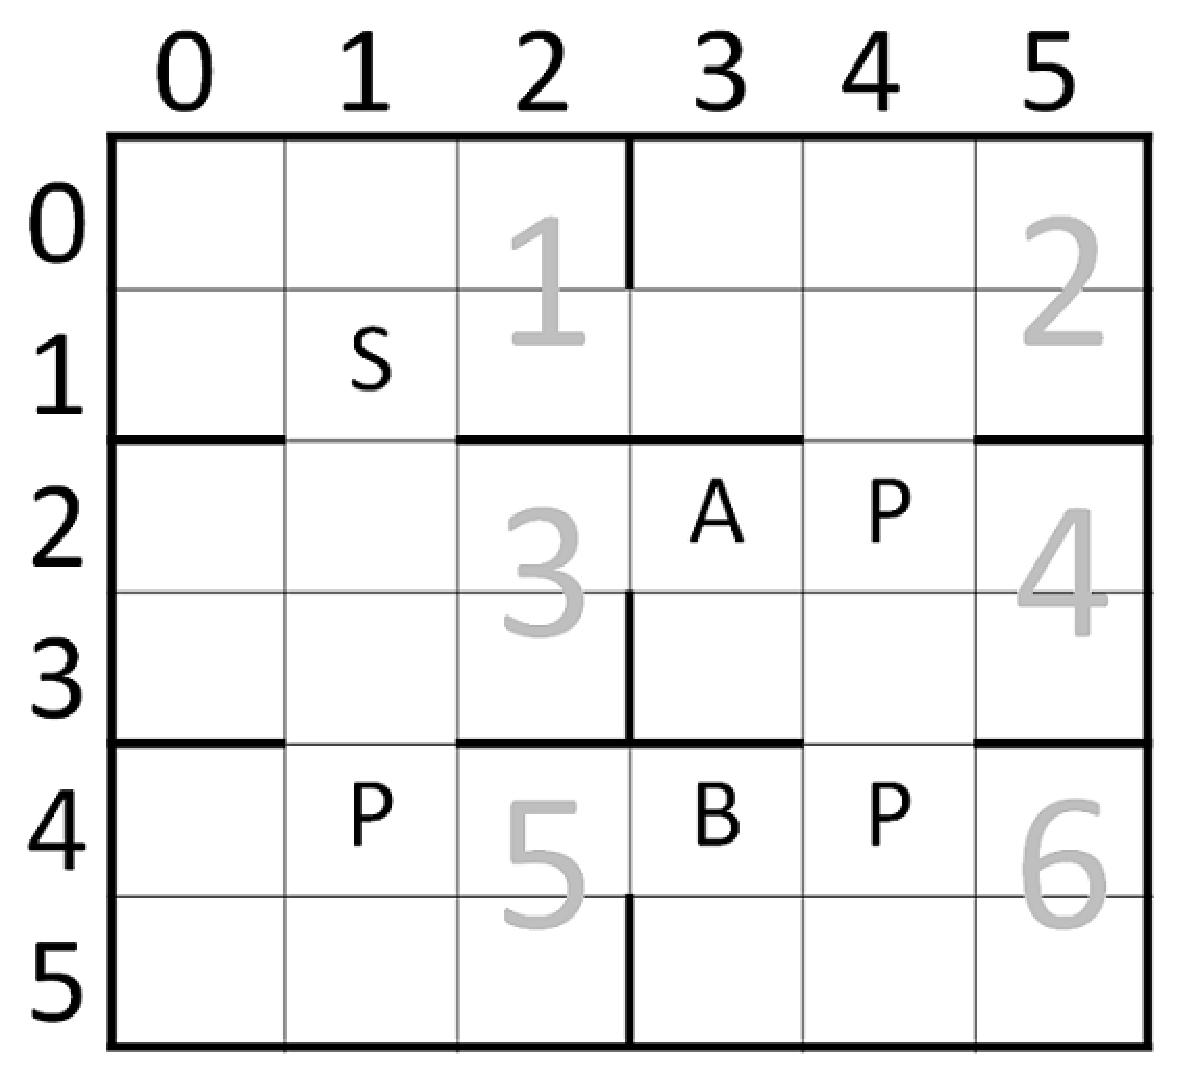
\includegraphics[width=2.5in] {BusSmall.eps}
    %\caption{(a)}
\end{minipage}
\begin{minipage}[b]{0.5\linewidth}
    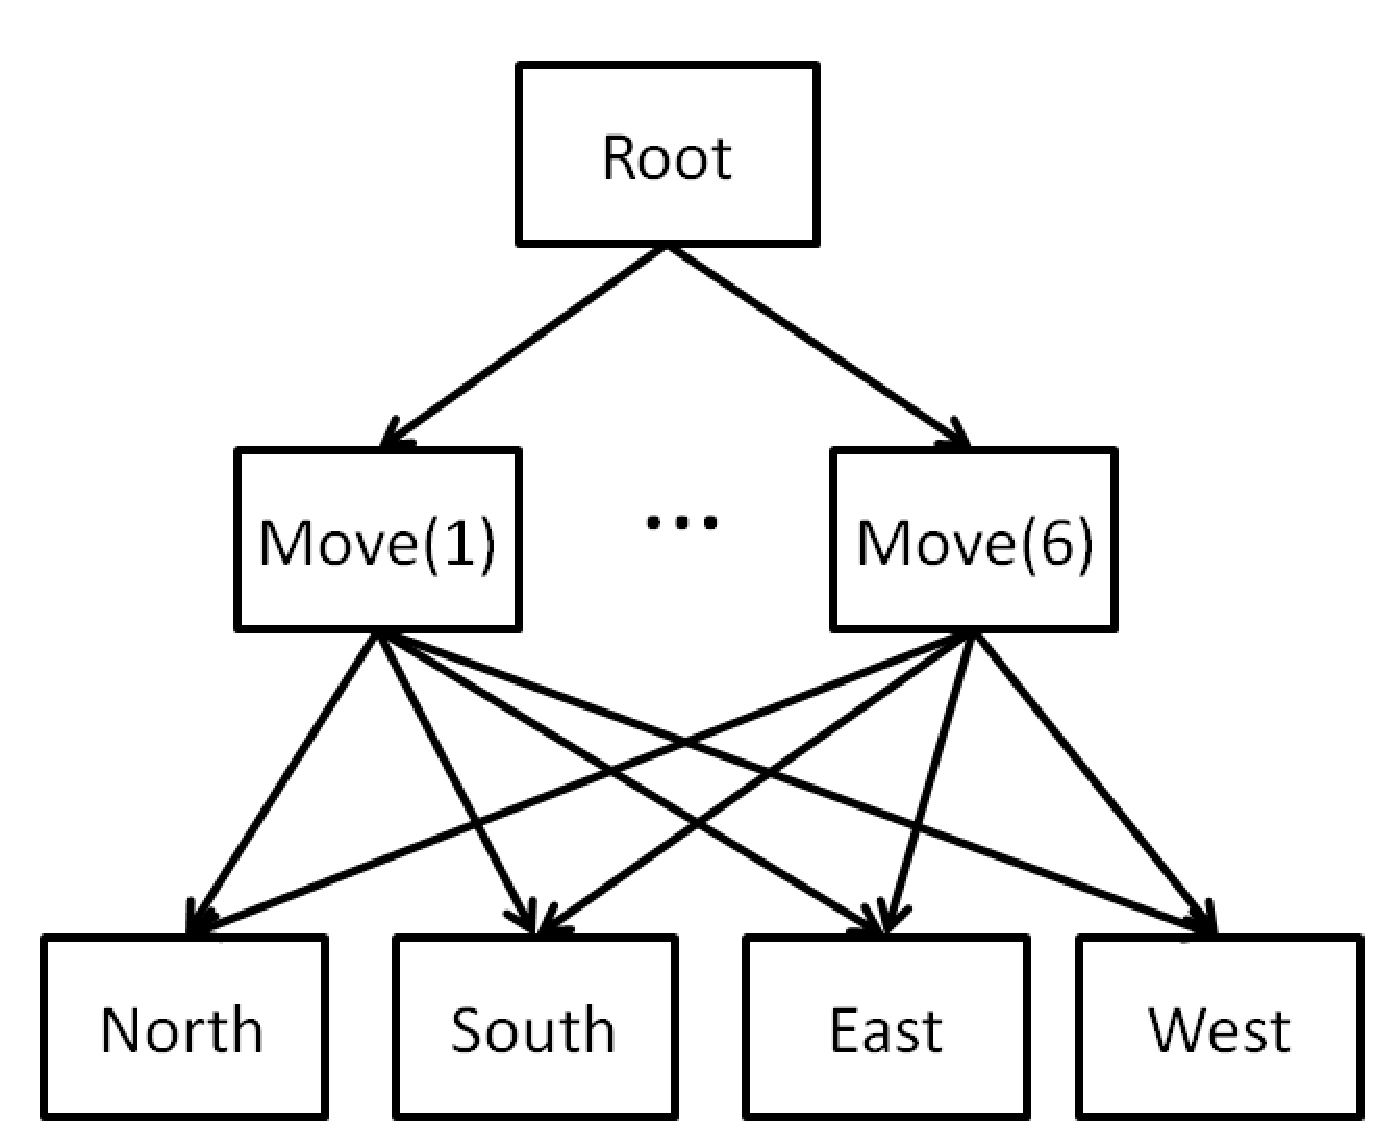
\includegraphics[width=2.5in] {BusHierarchy.eps}
\end{minipage}
\begin{minipage}[b]{0.5\linewidth} \centering (a) \end{minipage}
\begin{minipage}[b]{0.5\linewidth} \centering (b) \end{minipage}

%\end{center}
\caption{(a) The school bus domain (b) A task graph for the school bus problem.}
\label{fig:bus}
\end{figure}

We test our approach in the school bus problem. School bus starts at school $S$. Its task 
is to pickup all of three passengers marked as $P$ and return to the school(Figure \ref{fig:bus}a).
The episode ends when it finishes the task without extra reward. 
The passengers can be picked up in any order. The bus picks up the passenger automatically when it moves into
the location of passenger.

The bus can move North, South, East, or West. There is a reward of -1 for each action.
There is 0.1 probability for the bus to move in orthogonal direction. It stays put 
when trying to cross a wall. 

There are two locations which may be under road construction. They are marked as 
$A$ and $B$. If the bus pass any construction site, it will get damaged with probability 1 and has probability
0.25 to break down for each step. There is a reward of -50 if the bus breaks down and the episode ends immediately. 
At the beginning of episode, the status of road is randomly chosen from no construction, $A$ is under construction
,or $B$ is under construction. There is a 0.05 probability for the road status to change after the episode begins.


A state can be described by 8-tuple $(x, y, h, p_1, p_2, p_3, a, b)$, where $(x, y)$ is the location of 
bus, $h$ shows if the bus is damaged, $p_i$ indicates if the corresponding passenger has been picked up or not,
and $a$ and $b$ indicate the status of the construction sites.

%TODO: total leaf cover always exist
The task hierarchy is shown in Figure \ref{fig:bus}(b). 
The world is divided by 6 areas. Subtask $Move(t)$ moves the bus to area $t$. 
$Move(t)$ can only be invoked if $t$ is the adjacent area.
The subtask terminates if the bus exits the current area.
When it terminates, a pseudo reward $\tilde{r}$ is applied if the bus arrives designated area $t$ and 0 otherwise.

Since the six composite actions cover all primitive actions, they are a total leaf cover of the hierarchy.
We used HORDQ in their corresponding subtasks to guarantee the convergence to the optimal
policy. $Root$ subtask adopted our approximated model-based method. The planning variables include 
the location of bus and the status of passengers. The environment variables are the 
damage status of bus and the status of road. 

\begin{figure}[t]
%\begin{center}
 \begin{minipage}[b]{0.5\linewidth}
    %\includegraphics[height=11em, width=6em]{eli_bend.eps}
    \includegraphics[width=2.5in] {Approx.eps}
    %\caption{(a)}
\end{minipage}
\begin{minipage}[b]{0.5\linewidth}
    \includegraphics[width=2.5in] {Random.eps}
\end{minipage}
\begin{minipage}[b]{0.5\linewidth} \centering (a) \end{minipage}
\begin{minipage}[b]{0.5\linewidth} \centering (b) \end{minipage}

%\end{center}
\caption{The learning curve of the school bus domain, averaged over 400 episodes. (a) With our model-based approach. (b) With random planner.
The pseudo-reward is shown in the parentheses. The parameters are $\alpha=0.1$, $\epsilon=0.1$, and $\gamma=1$.
}
\label{fig:res}
\end{figure}

Our model learns when the bus is damaged, it will receive a large penalty.  
Since the damage status is assumed static during the planning process, 
it fails to learn that the bus will get damaged if it passes through
location $A$ and $B$. Our model is certainly biased in this case, and
it cannot learn the optimal policy. One solution is to include the damage 
status as one of the planning variables. However, the objective of 
the experiment is to show that the optimal policy can be achieved
with the biased model if we combine it with HORDQ. 



Figure \ref{fig:res}(a) shows the learning curves with different level of pseudo rewards.
With pseudo reward +60, it learned a suboptimal policy because
the pseudo reward is large enough to make $Move(t)$ subtask ignore 
the penalty of breakdown. As a result, The subtask followed 
the instruction of its parent strictly.

On other hand, if we do not impose any pseudo reward, 
the optimal policy can be learned, but the learning rate is
slower than flat SARSA learning. Since the subtask has no
incentive to follow the instruction from the hierarchy, 
the learning process is similar to flat SARSA learning 
except it has six different Q-functions to learn (one for each subtask) instead of one.
Thus it takes longer to learn the optimal policy. 

With appropriate pseudo reward, we can get a near-optimal policy
while the convergence rate is faster than flat SARSA learning.
Our experiment shows that a pseudo reward of +5 is enough to make subtask $Move(t)$ follow 
the order of $Root$ in most of the times, but it is not enough for the subtask to ignore
the breakdown penalty. When $Root$ executes $Move(4)$ to move the bus from area 
3 to area 4 and the road at location $A$ is under construction, $Move(4)$ subtask
will learn it is a bad decision with HORDQ.
Instead of moving to area 4, $Move(4)$ may move to area 1 or 5 to avoid
the breakdown penalty. In turn, $Root$ learns $Move(4)$ can not be done in 
such scenario, thus it will seek an alternate plan if the same scenario
is encountered.

The combination of our approximated model-based approach and MAXQ leads 
to a very poor result. MAXQ does not estimate the consequence of its action outside its own subtask, therefore
$Move(t)$ will follow the instruction of $Root$ at any cost.

To simulate the performance of the combination of poorly-approximated model-based method and 
HORDQ, we replaced our model-based approach with random one.
The result is shown in Figure \ref{fig:res}. In this case, flat SARSA learning has the fastest
learning rate. It takes more time for $Move(t)$ to realize that the policy of $Root$ is bad with higher pseudo rewards.
Nevertheless, it will eventually learn to a near-optimal policy.
The combination of random policy and MAXQ has the worst result.

The result shows that an good approximation model 
can help increase the learning rate with the combination of HORDQ. 
If the model is poor, HORDQ serves as a fail-safe mechanism to stop 
the agent repeating the same poor policy over and over again.

On the other hand, MAXQ learned a poor policy in both of cases.  

The result suggests us that in order to construct a robust HRL 
algorithm, it is beneficial to incorporate HORDQ in the hierarchy.

%On the contrary, the combination of MAXQ and a poor approximated model has
%a performance similar to random policy.

%TODO: add random agent experiment
%TODO: if I set the pseudo reward to zero, will the whole stuff breaks down again?

\section{Discussion and Future Work}
In this work, we propose a way to combine the approximated model-based method with the model-free
method (HORDQ) under the HRL framework. We are able to show that our approach can learn the optimal
policy even when the model is biased.  
Our work is general and can be combined with any model-based methods. 
A future direction is to investigate the applicability of combining our method with
other approximated model-based approaches.
%In this work we studied both object category and instance
%recognition using the RGB-D Object Dataset [14], a large
%RGB-D (color+depth) dataset of everyday objects. Our work
%is of interest both in terms of algorithm design and of
%the empirical validations on appearance and depth cues
%for recognition. Our key insight is that because a category
%consists of different objects, there is a natural division of a
%category into subclasses, and this motivates our use of the instance
%distance. We show that by jointly learning the weights
%in this distance function, we outperform alternative state-ofthe-
%art approaches. The proposed instance distance learning
%provides a distance measure for evaluating the similarity of
%a view to a known set of objects. This information can be
%used as input to other robotics tasks, such as grasping. An
%interesting direction for future work is to treat the training
%data as an object database where grasping information is
%stored for each object. When the robot encounters an object
%in the world, it can use the instance distance classifier



{\small
\bibliographystyle{plain}
\bibliography{biblio}
}
\end{document}

\endinput
